\chapter{肺部球形病灶}

肺部球形病灶在X线胸部摄片上形成肺部圆形阴影,其原因较多(表\ref{tab9-1}),较常见的是结核球、周围型肺癌,其次为肺脓肿、各类肺内肿瘤、炎症机化、肺寄生虫病等。这些肺部圆形阴影从临床上与X线影像学上有时难以确定其性质,但依靠病灶所在部位及其形态、边缘、密度和病灶附近肺野的改变,观察病灶发展过程中所形成的各种征象,结合临床表现和各种检查资料进行综合分析,常能获得较为正确的诊断。

\begin{table}[htbp]
\centering
\caption{肺部球形病灶疾病的分类}
\label{tab9-1}
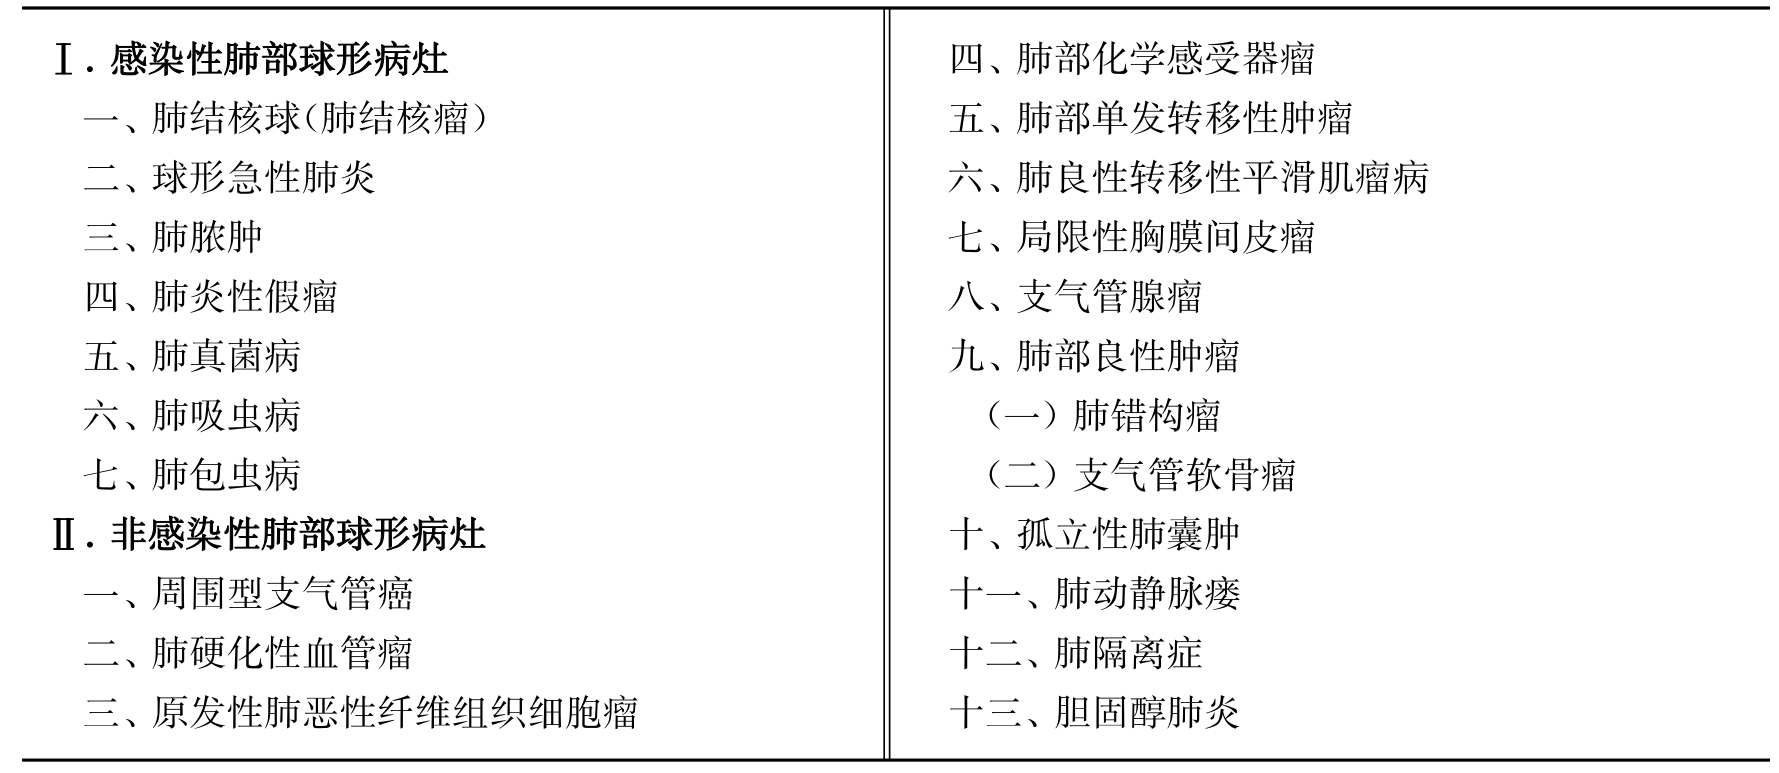
\includegraphics[width=5.91667in,height=2.57292in]{./images/Image00065.jpg}
\end{table}

\section{【肺部病灶与肺外病灶的鉴别】}

在X线胸片上,主动脉瘤与胸壁淋巴结结核最易与肺部球形病灶相混淆,须首先区别之。

主动脉瘤多发生于升主动脉,也可发生于主动脉弓及降主动脉,在X线胸片上呈圆形或卵圆形、边缘光滑清晰的阴影,形状、大小不一,其特点是与主动脉相连并有扩张性搏动。病因多为梅毒性。升主动脉瘤多有明显的体征,而临床症状轻微,曾有“只有体征的动脉瘤”之称。在心底部,尤其是胸骨柄部位有时可触及异常的搏动、叩诊呈异常的浊音或实音。如异常搏动与浊音同时出现于胸骨右侧,诊断意义较大。动脉瘤上可有收缩期震颤与杂音。动脉瘤如侵蚀胸骨与肋骨,可在皮肤下形成一隆起的圆形肿块。弓部主动脉瘤最常引起压迫症状。由于主动脉弓后面有气管、食管和交感神经丛,此外尚有喉返神经环绕,而左侧膈神经又与其前壁密切接近,故弓部主动脉瘤早期便可产生压迫症状,因而有“多症状动脉瘤”之称。当气管或左支气管受压时,可发生一种吼哮样刺激性咳嗽。若左喉返神经受压,则出现发音困难与声音嘶哑。食管受压则引起吞咽困难。交感神经受压,可发生双侧瞳孔大小不等。膈神经受刺激时可引起呃逆,持续受压时可引起左膈麻痹。患者有时可发生气促,主要由于支气管受压与肺不张所致。肺主动脉瘤须经X线和血管超声多普勒检查或血管造影确诊,但有时不易与纵隔肿瘤相区别。

胸壁淋巴结结核在X线胸片上常显示圆形阴影,易被误诊为肺内病变。如有下列的情况,可协助鉴别:①圆形阴影在X线透视下深呼吸时与肋骨移动一致;②侧位或斜位照片时,可见此阴影呈半球状与胸壁密切接触;③做诊断性人工气胸术时,如发现胸膜粘连,也有助于与肺内病变相区别;④薄层CT扫描对诊断帮助更大。

此外需注意包裹性胸腔积液、纵隔肿瘤、先天性膈疝、胸膜肿瘤等与肺部球形病灶相区别。

\section{【“良性”病灶与恶性病灶的区别】}

“良性”肿物的圆形阴影,其边缘往往光滑而清晰,但有些恶性肿瘤如周围型支气管癌、淋巴肉瘤及纤维肉瘤,其边缘有时也可光滑。恶性肿瘤的边缘大多数模糊,呈毛刺状、多叶状,但有些“良性”病灶如肺炎球形病灶、肺脓肿浸润期、肺结核球等,其边缘也可模糊。肺包虫病和结核球也可呈分叶状,因而须密切结合临床及其他有关检查进行诊断。

有钙质沉着的球形病灶多属“良性”,常见于肺错构瘤、肺结核球、肺包虫病等。但瘢痕癌、某些肺癌的病灶也有钙化点,因此,不能单凭有无钙化点来判断良恶性。

可随呼吸而改变形态的圆形阴影,多为壁薄而内含液体的囊性肿物,如肺包虫囊肿与肺动静脉瘘。前者为地方性寄生虫病,后者常有发绀、杵状指(趾)等表现。如肺圆形阴影上方有半月状透亮区,可见于肺包虫囊肿、肺曲霉肿、肺脓肿、肺结核球等。

恶性球形病灶通常有进行性增大的特点,可从小病灶发展成为大的球形或不规则形病灶,当球形病灶直径增加28\%时,肿块重量增加一倍。肿块倍增时间一般为25~450天,平均120天。而“良性”肿瘤一般增长缓慢,长时期改变不明显。快速增长的也是良性病变的特征,如炎性结节和肿块。偶尔也有增长相当缓慢的支气管肺癌。恶性肿瘤多有进行性消瘦、厌食等表现,而“良性”者症状缺如或轻微。恶性肿瘤的肺转移,常表现为多发性大小不等的圆形阴影。肺部球形病灶良恶性鉴别见表\ref{tab9-2}。

\begin{table}[htbp]
\centering
\caption{肺部球形病灶良恶性的鉴别}
\label{tab9-2}
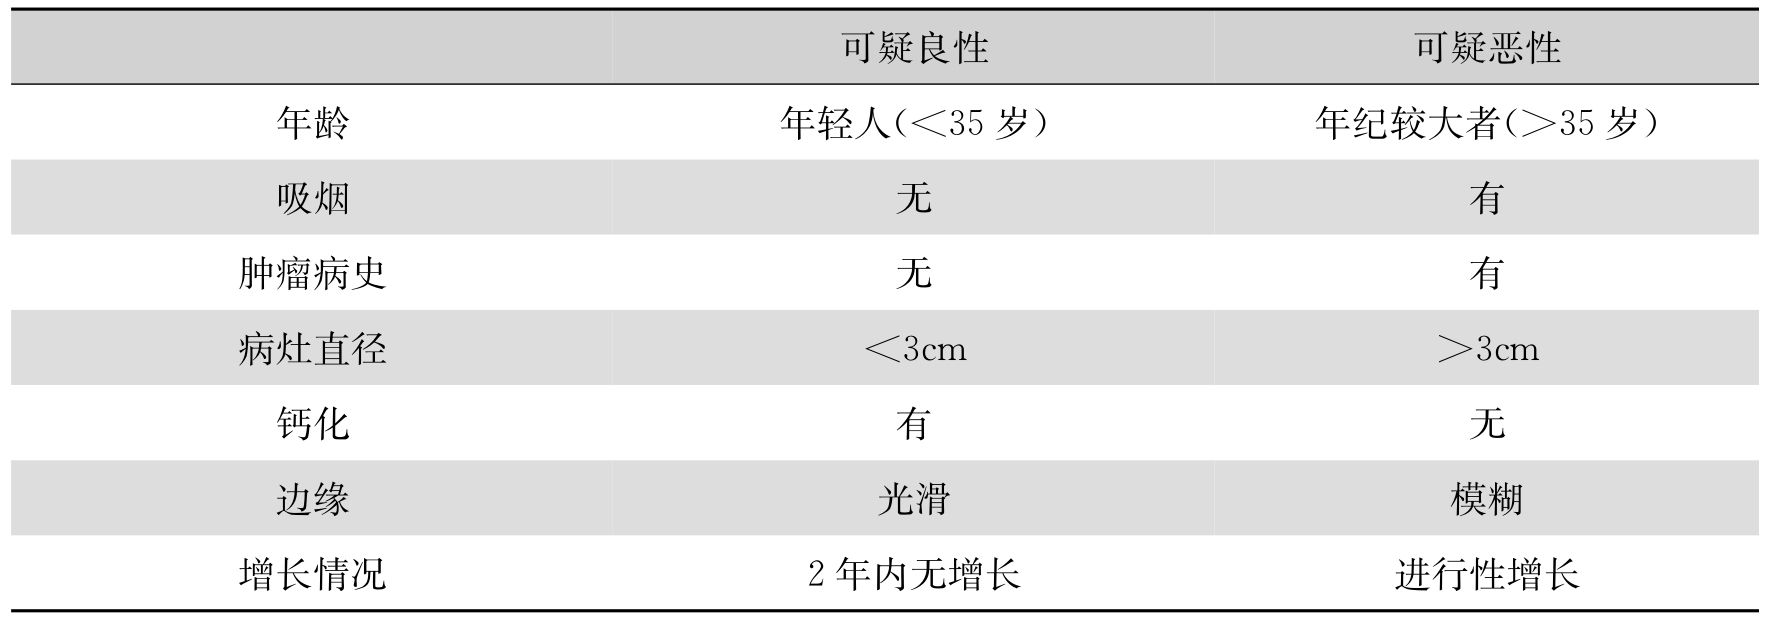
\includegraphics[width=5.90625in,height=2.08333in]{./images/Image00066.jpg}
\end{table}

如经各项检查,而肺部球形病灶未能除外恶性,若无手术禁忌证,应及早经皮肺穿刺活检或开胸探查。

\protect\hypertarget{text00089.html}{}{}

\section{30 感染性肺部球形病灶}

\subsection{一、肺结核球(肺结核瘤)}

在肺部球形病灶中,肺结核球所占的百分率最高,肺结核球以单发性为最多见,有时也有多发性。结核球直径多在2~4cm以内,超过5cm者颇少。结核球虽可发生于任何部位,但位置多偏后,常见于两上肺尖后段,其次为下肺背段及后基底段,其他位置则很少见。据报道,结核球发生在两肺上叶尖后段和下肺背段者占93
5\%。

结核球发病年龄在20~60岁,40岁以上并不少见。男性多于女性,男∶女为4∶1,约半数患者无明显的自觉症状,其余有咯血、胸痛、肩背痛、咳嗽、低热、乏力、体重减轻、盗汗等症状。痰找结核菌约5\%~30\%阳性。结核菌素皮内试验强阳性有助于诊断与鉴别诊断。

肺结核球在X线影像表现可归纳如下:

(1)肺结核球为干酪性病灶,外围有一纤维包膜,因而球形病灶边缘一般清楚而光滑;当结核球在浸润进展时其边缘可变为模糊或不整齐。

(2)结核球多为中等密度且多不均匀,内部常有钙化物质,可呈同心环形、弧形钙化或斑点小结节状钙化,此为结核球的特征性表现。结核球内钙化越多意味着病情趋于稳定。

(3)肺结核球内可有空洞形成,多偏向肺门一侧。

(4)肺结核球邻近的肺野多有结核病灶(卫星灶),并有支气管引流征引向肺门,呈细长条状密影与肺纹理平行;且常有局部胸膜增厚粘连,一般无肿大的淋巴结。

这些有价值的X线征象在结核球的鉴别诊断时要注意识别。

CT、高分辨率CT(HRCT)、MRI可更清楚的显示病变特性,有学者认为同层动态CT增强扫描,对肺内孤立性结节(SPN)的定性诊断有较大价值,并将SPN的净增值<20HU作为良性结节的阈值指标。肺结核瘤通常引起对\textsuperscript{18}
F-氟代脱氧葡萄糖(\textsuperscript{18}
F-FDG)的摄取增强,故在结核好发部位的病灶,\textsuperscript{18}
F-FDG正电子发射计算机体层扫描(PET)显像阳性者,应注意与肺内恶性肿瘤鉴别。

肺结核球的诊断主要根据病史、症状及上述X线影像学表现,结合结核病化验检查的阳性结果,通常不难与肺部其他球形病灶如周围型支气管癌、肺包虫病、肺脓肿、肺错构瘤等相鉴别(参见下文)。

由于胸膜皱缩阴影、病灶不超过叶间胸膜并不是肺癌独有的征象,也见于结核球和炎性假瘤,因此,对这些疑难病例的确存在鉴别诊断困难时,若无手术禁忌证,应早期进行有创检查或手术治疗。

\subsection{二、球形急性肺炎}

球形肺炎是肺炎的一种特殊表现形式,病原体可为病毒或细菌、真菌(见下述肺真菌病),多为肺炎链球菌和葡萄球菌,误诊率较高,常被误诊为肺结核瘤或肺癌。患者起病急,伴发热、咳嗽、咳痰,外周血白细胞增多等急性炎症表现,亦有无症状及(或)白细胞不多者。如为肺炎链球菌,其尿抗原可阳性。X线表现为孤立的圆形,椭圆形病灶;病灶中央密度较高,边缘密度低,呈晕轮样改变;病灶边缘纹理明显增粗,即所谓“胡须征”。X线胸片鉴别困难时,胸部CT、纤维支气管镜检查可帮助鉴别。抗生素治疗1~2周,如病灶吸收、好转,可作为诊断肺炎的可靠依据。

球形肺炎主要与下列疾病鉴别:

\subsubsection{(1)肺内结核球:}

边缘清晰,锐利,密度较高,多有钙化,邻近肺野有卫星病灶,不增强或包膜样增强。抗结核治疗有效,结合临床可与之鉴别。

\subsubsection{(2)肺梗死:}

梗死灶多呈基底朝向胸膜侧的楔形,且常伴有胸膜反应。

\subsubsection{(3)机化性肺炎及炎性假瘤:}

两者抗炎治疗无效,而球形肺炎治疗后可完全吸收或仅遗留少许索条影。

\subsubsection{(4)周围型肺癌:}

①球形肺炎CT表现病灶边缘毛糙且模糊,可见粗长毛刺,有时呈浅分叶,可见“晕轮征”。周围型肺癌边缘清晰,呈深分叶,有细毛刺,不见“晕轮征”;球形肺炎多为方形或三角形,而周围型肺癌多呈类圆形或卵圆形,不见方形。②有报道良性结节平扫CT值低于恶性结节,增强扫描结核的CT值增加值<20HU,炎症和癌肿均呈明显强化(20~70HU或更高),不易鉴别,但后两者的动态CT扫描有所不同,前者时间-密度曲线呈双峰型,后者呈单峰型,且峰值低于前者。③球形肺炎肺纹理可贯穿病灶,而肺癌很少有此征。④球形肺炎病变所属支气管黏膜充血水肿,周围型肺癌如累及支气管则主要为受累支气管不规则狭窄,纤支镜查可见受累支气管内有新生物。⑤球形肺炎极少有肺门及纵隔淋巴结增大,周围型肺癌比较多见;球形肺炎常出现胸膜增厚、粘连或少量积液,而肺癌则相对少见;球形肺炎抗炎治疗多有明显缩小,而周围型肺癌抗炎治疗无效。

\subsubsection{(5)严重急性呼吸综合征(SARS):}

亦可表现为球形肺炎,由SARS冠状病毒引起的一种全新的急性传染病。其临床特征为:①有明显的传染性,接触患者后起病,或群体起病,或作为传染源。②潜伏期为2~10天,大多数为4~5天,抗菌药物无效。③大多数患者以发热为首发症状,多为高热,可有畏寒、伴或不伴有头痛、关节酸痛、肌肉酸痛、乏力、胸痛、部分患者有腹泻。部分患者快速发展至呼吸衰竭,发热至出现呼吸困难的中位时间为5天(3~7天)。④呼吸道症状多在中后期出现,表现为咳嗽、偶有血性痰;严重者出现呼吸困难,个别进展为急性呼吸窘迫综合征。⑤肺部体征多不明显,部分患者可闻少许湿啰音。患者的呼吸道症状和肺部体征与胸部X线的表现相比常常较轻。⑥早期血白细胞计数不升高或降低,淋巴细胞计数减少。⑦胸片进展迅速,多数从单侧球形病灶发展为双侧。

SARS患者胸部平片和CT影像特点为病灶开始为单发球形或斑片灶,以后迅速进展为多个病灶,甚至双肺多发病灶,以周边部位多见。文献报道70\%病灶远离肺门,位于周边部位,27.5\%病灶同时累及周边和中心,2.5\%发生在中心部位。病灶密度以磨玻璃样改变多见,占62.5\%,实变占17.5\%,两者均出现者占10\%。形态以斑片和球形最常见,占82.5\%。以下叶外段、背段、前段,中叶(舌叶)和上叶前段的分布多见。

SARS的诊断应根据流行病史、临床、实验室和影像检查的综合判断。SARS患者胸部影像表现本身不能单独做出诊断,但认识SARS患者胸部的影像特点非常重要,有助于疾病的鉴别。

\subsection{三、肺脓肿}

肺脓肿在X线胸片上可呈圆形或卵圆形阴影,常为单发性,有时为多发性。常有脓腔形成,脓腔周围多伴有不同程度炎症浸润,脓腔内可有液平面,病灶边缘模糊而不规则。CT能更清楚的显示病灶形态、大小、数目、密度及其周围、肺门及纵隔淋巴结、支气管形态结构、少量胸腔积液和胸膜增厚等,有助于诊断。患者起病时多有畏寒或寒战、发热,继而咳出脓性而有臭味的痰或血性痰。血象白细胞增多。在脓腔周围炎症吸收后,较小的脓腔自行愈合,腔壁纤维化,而较大的脓肿则常不易愈合,成为慢性肺脓肿。

有些肺脓肿在X线胸片上呈边缘清楚的圆形阴影,或肺脓肿的引流支气管受阻、脓液不能排出,形成圆形阴影而酷似支气管癌,须加以区别,主要根据:①肺脓肿常以寒战、发热等全身感染症状起病,而支气管癌则无明显的全身症状。②支气管癌的边缘较肺脓肿略清楚,周边毛刺较短,形成空洞的可能性不多;如形成空洞,多呈偏心性,洞壁厚薄不均,内缘凹凸不平,多无液平面,与肺脓肿的多个空洞互相通连及内壁光滑的形象不同。③癌瘤如发生在肺叶边缘,时常为叶间隙所限而不跨叶,并有将叶间裂推移现象;反之,肺脓肿则因纤维化与瘢痕形成而收缩,对叶间裂有牵拉现象。④肺脓肿周围有较多的纤维条索状病变,邻近肺组织内常有不规则的扭曲的细条阴影或有胸膜增厚与粘连现象。如支气管肺癌有肋骨转移,临床出现肋骨压痛,X线检查可发现侵蚀缺损区,有助于支气管癌的确诊,但此已属癌症后期征象。

肺脓肿的脓腔内如有陈旧性血块,或坏死组织形成团状,游离于脓腔中,可随体位而移动,并形成半月形透亮区,酷似肺曲霉肿,但曲霉肿周围的肺部炎症、纤维化及支气管扩张皆较少见。

\subsection{四、肺炎性假瘤}

本病少见,多发生于21~50岁的成年人,常见的症状是痰中带血丝、咳痰、发热与胸痛,消瘦也较多见,但也可无症状。X线胸片所见多为边缘清晰的圆形阴影,多为单发,偶有多发;一般不侵犯周围肺组织与胸膜;病灶大小不一,罕见钙化。CT显示肿块内单个或多个小空洞,周围少量粗长索条状毛刺,病变的某一层面可见一侧边缘垂直于胸膜呈刀切样改变,胸膜增厚粘连征象对本病诊断有着重要意义。此种阴影可经积极的抗菌药物治疗,而于短期内逐渐消散;但如炎症病灶已机化,往往此阴影呈长期静止不变的良性经过。

纤维支气管镜、CT引导下肺穿刺活检有助于诊断,但术前诊断比较困难,往往需开胸手术病理确诊。肺炎性假瘤与周围型支气管癌不易区别,且有癌变的可能,因此主张放宽手术指征。

\subsection{五、肺真菌病}

\subsubsection{(一)肺曲霉肿(亦称肺曲菌球)}

大多继发于肺结核空洞、支气管扩张症、肺脓肿、肺囊肿、肿瘤化疗后、使用免疫抑制剂后,或机体免疫力低下的基础上,原发性感染少见。患者可出现咳嗽、咳痰、发热、盗汗、乏力和纳差等症状,慢性者症状类似肺结核,可出现咯血等症状,与患者原有的慢性肺部病变的症状不能鉴别,易导致误诊。

如慢性肺结核患者,长期应用抗结核药物治疗,痰结核菌虽已阴转,但空洞仍持续存在或扩大,X线显示空洞内有密度不太一致的圆形或卵圆形块状阴影,临床症状除反复间断痰中带血或咯血外,无发热、胸痛、气急等症状,提示肺曲霉肿的可能性。

曲霉肿好发于上叶,位于下叶者甚少,由曲霉丝混合成球形(曲霉可为活的、死的或已钙化的菌块),寄生于病灶空洞或囊状扩张的支气管腔内,曲霉肿与洞壁之间可见一半月形透亮带,该透亮带可随患者体位的改变而移位。如采取多种体位作X线摄片检查,可显示曲霉肿和透亮带的移动性,此为曲霉肿特征性改变。CT薄层扫描比X线更易发现病灶内的小空洞,有利于提高诊断率。

\subsubsection{(二)侵袭性肺曲霉病}

是肺真菌感染最常见的类型,症状以干咳、胸痛常见,部分患者有咯血。早期胸部CT表现为结节或肿块样阴影,外周有一日晕样环状阴影,其密度低于中央的肿块,但高于周围正常肺组织,称“晕轮征”,是早期确诊的首要征象,后期由于组织坏死可出现“新月体征”。

肺曲霉病的确诊有赖于组织培养(病变器官活检标本)及组织病理学检查,镜检可见锐角分支分隔无色素沉着的菌丝,直径约2~4μm;无菌组织或体液培养有曲霉属生长。如呼吸道标本(痰液、支气管肺泡灌洗液和支气管毛刷)镜检真菌成分显示为霉或培养阳性;或肺、脑、鼻窦CT或X线有特征性改变;患者为免疫抑制宿主应怀疑曲霉病。血、尿、脑脊液及肺泡灌洗液曲霉半乳甘露聚糖测定(GM试验)和PCR测定血中曲霉DNA对本病诊断亦有帮助,动态观察其变化对诊断更有价值。

本病主要与肺结核球和周围型肺癌的空洞相鉴别。肺结核球常发生于上叶尖后段或下叶背段,周围常有卫星灶,洞较大,壁薄,空洞内容物可为干酪坏死团块,密度不均,边缘不规则,无移动性。周围型肺癌空洞,壁厚不均,外缘呈分叶状,洞壁球形结节形态不规则,不能移动。查痰找到结核菌或癌细胞有助于鉴别。而肺曲霉肿的X线表现是空洞或空腔内的球形阴影,密度均匀,边缘清楚,位置可随体位移动;侵袭性肺曲霉病则球形阴影有动态的变化。肺活检找到曲霉有意义。

\subsubsection{(三)肺隐球菌病}

患者临床表现无特异性,多以咳嗽、咯血为主要症状,亦可有发热、胸痛。甚至可无任何症状,胸部影像学表现多样,往往须经手术探查方能确定诊断。病变下肺多于上肺。X线胸片病灶大多呈块状或球形阴影,部分有分叶或毛刺现象,也可呈小结节状或片状渗出阴影。血清隐球菌抗原阳性,经皮穿刺活检、纤支镜检和开胸探查病理确诊。

\subsection{六、肺吸虫病}

肺吸虫病是由于肺吸虫幼虫在肺内游动、成长和产卵形成的疾病。流行于亚洲东南部。我国见于浙江、台湾、长春及延边等地区。临床表现多有咳嗽、胸痛、咯血或咳果酱样痰;痰中可查到肺吸虫卵。

肺吸虫病的诊断线索是相应的流行病学史与咯血痰。肺吸虫病的囊肿期,常呈散在性单体囊肿,在X线胸片上呈圆形或卵圆形阴影,其大小不一,直径约为1~2cm,数目不定,从1个至10多个,病变多位于中、下肺野。典型的肺吸虫病X线征为囊肿边缘清晰或有些模糊,密度均匀,与软组织大致相同的结节状阴影。肺吸虫囊肿的壁随着病程的发展可变得更厚和致密,其液状内容物密度相对地降低------这种病理变化在X线摄片上即显示出环状壁以内的、密度减低的空泡状阴影。此等密度较高的环状阴影或含有多发性小透亮区的结节状阴影是肺吸虫病的X线特征。

本病的囊肿与肺结核球液化所形成的空洞的区别点为:肺吸虫所引起的囊状阴影密度较低,内有空泡而罕见有钙化点,多位于中、下肺野;肺结核球则多发生于中、上肺野,阴影密度较高,常有钙化点存在,球形病灶周围有结核病灶存在。肺转移性肿瘤、良性肿瘤常呈密度均匀的结节状阴影,而周围常无肺吸虫病所致的浸润性或纤维性阴影,也无空泡状阴影。

有生食或半熟食蟹、虾、蝲蛄史;有发热、胸痛、咳嗽、咳铁锈色痰等症状;结合特征性X线胸片改变、外周血嗜酸性粒细胞增多需注意肺吸虫病。肺吸虫抗原皮内试验及(或)循环抗体测试阳性、皮下结节活检均有助于确诊。

\subsection{七、肺包虫病}

肺包虫病主要见于我国西北及内蒙地区,此病在无并发症时常无明显自觉症状,而多在健康检查胸部透视时发现。由于包囊胀大压迫支气管而引起狭窄及部分肺不张,或并发支气管扩张,患者可有胸部不适、咳嗽、咳痰及劳动后气短等症状。包囊破裂可发生咯血,如合并细菌感染可形成肺脓肿。

胸部X线检查在无并发症的肺包虫囊肿,皆呈圆形或卵圆形、略呈分叶状的阴影,边缘清晰,密度均匀,如继发感染则边缘不齐。较大的包虫囊肿在透视时偶可见随深吸气时从圆形变为长圆形,呼气时恢复原状的变形现象。陈旧的肺包虫囊肿在X线胸片上可发现囊壁有钙盐沉着,个别患者甚至完全钙化呈蛋壳样。包虫抗原皮内试验(Casoni试验)、补体结合试验及酶联免疫吸附试验对此病有重要诊断意义,阳性率可达90\%以上。

B超、MRI等检查有助于本病的诊断,CT扫描能发现普通胸片难以显示的纵隔隐匿性肿块,还能根据组织密度或衰减作出定性诊断,并可反映子囊的存在。CT检查结合Casoni试验可使肺包虫病的诊断达到相当高的精确度。

单个的圆形包虫囊肿须与肺结核球相区别,二者皆可发生于年轻人,后者密度较包虫囊肿高,边缘整齐,不随呼吸而变形,增长较慢;肺包虫囊肿阴影常比肺结核球更大,增大较快,其钙化影皆位于囊肿壁上,囊肿形态可随呼吸而变形。如空气进入内囊与外囊之间,则呈现一半月形透亮带。如内囊破裂,空气进入内囊,可见除有一液平外,其上方有二弧形透亮带。如内囊破裂塌陷而脱落,则形成不规则的膜状物,漂浮于液面而在X线胸片上观察到。如包虫囊轻微破裂,呈一有空洞状阴影,易误诊为肺脓肿;经过2~3个月后囊内气体被吸收而恢复圆形阴影。如液体全被排出,在原包囊位置遗留下肺组织纤维化阴影。

肺包虫病与周围型支气管癌的X线影像相类似,但如发现有钙质沉着,则支气管癌的可能性甚少;在高电压或超高电压的摄片上,包虫囊肿影像几乎消失,但支气管癌的阴影仍常存在。此外支气管癌生长快,病程短,边缘不清,呈毛刺状。肺转移性癌在X线胸片上常呈多发圆形阴影,其大小相差不大,生长快而症状明显。原发癌的发现,癌细胞学检查及支气管造影检查,对肺转移癌的诊断有较大帮助。

根据患者有羊、狗接触史,包虫三项试验(Casoni试验、补体结合试验及酶联免疫吸附试验)阳性,结合临床表现及胸部X线、CT特征,进行综合分析,多能作出正确诊断。

\protect\hypertarget{text00090.html}{}{}

\section{31 非感染性肺部球形病灶}

\subsection{一、原发性支气管肺癌}

在肺部球形病灶中,原发性支气管肺癌(肺癌)占相当数量。肺癌由于生长部位、病理特点和X线表现不同,一般分为中央型及周围型肺癌两类;在肺部呈圆形阴影者以后者为多见。周围型肺癌的主要X线表现为:①肺内孤立性球形病灶;②边界清楚且具有不同的毛刺状阴影;③轮廓可呈凹入或作分叶状;④肿块密度均匀,一般无钙化;⑤少有空洞形成;如有空洞,通常呈厚壁、偏心性、内腔凹凸不平,并有突入空洞的结节而多无液平面;⑥周围型肺癌邻近肺野内可出现小节段性肺炎和肺不张,并可随癌增长而逐渐增大或反复出现。

支气管造影检查对周围型肺癌的诊断有一定价值,可补充平片及支气管镜检查不足之处。其造影征象表现为:①截然的阻塞,其断面可能为斜向或横向,光滑或不规则,凸出或凹入;②鼠尾样不规则的缺损;③侧壁的不规则缺损;④某一分支的缺如。应该指出,此等缺损仅在其他肺段支气管直至末梢均充盈良好,而缺损分支与平片所见阴影相一致时方有意义。但随着CT、MRI和PET相继出现,此项目检查已逐步被取代。

恶性肿瘤组织对67镓有极大的亲和性,而对其他组织则否,静脉注入后作肺扫描,直径在2cm以上的肺癌病灶可清晰显示,据此可与其他“良性”肿块相区别。

某些特殊检查有助于周围型肺癌的诊断与鉴别,如:①新的分子病理学技术能在痰中找到ras及(或)p53突变基因;一种单克隆抗体(Mab
703D4)对识别痰标本中的肿瘤抗原具有较高的特异性和敏感性,可提高早期确诊率。②经纤维支气管镜肺活检,纤支镜细胞刷片检查,CT导向下经皮肺穿刺活检,锁骨上肿大淋巴结活检有助于确诊。纵隔镜、胸腔镜活检也有一定价值。③高分辨率CT能发现常规胸片不能显示的小的周围型结节病灶,配合纤支镜或针吸活检多能确诊。④正电子发射计算机体层显像(PET)可探查局部组织细胞代谢有无异常。与正常细胞相比,肺癌细胞的代谢及增值加快,对葡萄糖的摄取增加,作为反映葡萄糖在肿瘤细胞内代谢的标志物,注入体内的\textsuperscript{18}
FDG相应地在肿瘤细胞内大量积聚,其相对摄入量可以反映肿瘤细胞的侵袭性及生长速度,故PET可用于肺癌及淋巴结转移的定性诊断。⑤肿瘤标志物配合影像学改变,可以帮助诊断。当然,确诊有赖于组织病理诊断,如经皮肺活检、内科胸腔镜等。

肺癌形成球形病灶而瘤体不大时最易被误诊为肺结核球。误诊原因主要为症状(如咳嗽、咯血、胸痛、微热)和X线征象类似,肺癌痰中癌细胞阳性率与结核球结核菌阳性率都不高,且肺结核与肺癌同时存在的情况易被忽略。但从患者的年龄、症状、病灶的部位、大小、形态等可以鉴别:①肺癌多见于40岁以上,而结核球多见于40岁以下;②肺外症状可作为肺癌的辅助诊断指标,而结核球罕见,肺外表现重要意义在于这些表现可出现在肺癌被发现之前周或数月;③肺癌好发于肺的前方(上叶前段、中叶、舌叶),而结核球好发肺的后方(上叶尖后段、下叶背段);④肺癌在确诊时多数病例的病灶已超过3cm,结核球多在2~4cm以内;⑤肺癌的球形病灶边缘有毛刺,分叶状,钙化较少,病灶内有空泡征(为肿瘤在细支气管肺组织内散在生长或肿瘤细胞伏壁生长,肺泡产生较多的空隙),而结核球、炎症假瘤和良性肿瘤未见空泡征象;⑥病灶周围卫星灶,结核球占73.1\%~86.6\%,其内伴有钙化卫星灶者占25.5\%,而肺癌仅占3.0\%~7.0\%,肺癌的卫星灶除少数为癌性转移外,大部分为散在硬结钙化灶,炎性假瘤和错构瘤均未见卫星灶。说明结核球常可见较多的卫星灶,而周围型肺癌绝大多数无卫星灶。

孤立性周围型肺癌与肺结核球、肺良性瘤、肺转移癌、肺脓肿等鉴别见表\ref{tab9-3}。如肺部圆形阴影经各项检查仍未能确定原因,也未能除外肺癌的可能性,无禁忌证时应及早开胸探查。

\subsection{二、肺硬化性血管瘤}

肺硬化性血管瘤(PSH)是一种低度恶性肿瘤。通过免疫组化和电镜对PSH研究证实,PSH是一种向Ⅱ型肺泡细胞分化的上皮细胞。多见于青中年女性,50\%~87\%的患者无临床症状,少数可有咳嗽、咯血、胸痛等症状,也可伴有间歇性低热、乏力等。X线胸片呈孤立性、边缘清楚、密度均匀、圆形或类圆形结节状阴影,少数可有浅分叶状,但多为边缘光滑、锐利,且无肺门及纵隔淋巴结肿大。也可为多发性。右肺多于左肺,一般以中下叶为多,直径多在1~3cm。CT扫描常示密度均匀的软组织阴影,但肿瘤有囊性变时可呈低密度区。增强扫描时肿块密度均匀或不均匀强化,少数病例可见“新月体征”。CT及增强扫描对本病的诊断有重要意义。甲状腺转录因子-1(TTF-1)及上皮膜抗原(EMA)等免疫标记对PSH的诊断具有重要的价值。细针活检做细胞涂片及免疫组化检查有时可获得诊断,手术仍是诊断和治疗该病的主要方法。

手术中见病灶周围有假包膜包裹。病灶密度多较均匀,其内少有钙化灶,若瘤体破裂出血,并与支气管相通,可出现空气半月征。

\subsection{三、肺原发性恶性纤维组织细胞瘤}

该瘤曾称纤维黄色肉瘤,多发生于四肢及软组织,原发于肺者少见,好发于中、老年人,男性明显多于女性。临床症状无特异性,患者可有咳嗽、咳痰、痰带血丝、胸背疼痛等症状。此瘤以右肺上叶较多见,多呈分叶结节状团块,边界较清,易被误诊为炎性假瘤、肺癌、肺转移瘤、结核瘤或良性肿瘤。仅靠临床表现难以明确诊断,因此诊断主要根据肺活检和手术后标本病理学检查。

\begin{table}[htbp]
\centering
\caption{几种肺野内球形病灶疾病的鉴别}
\label{tab9-3}
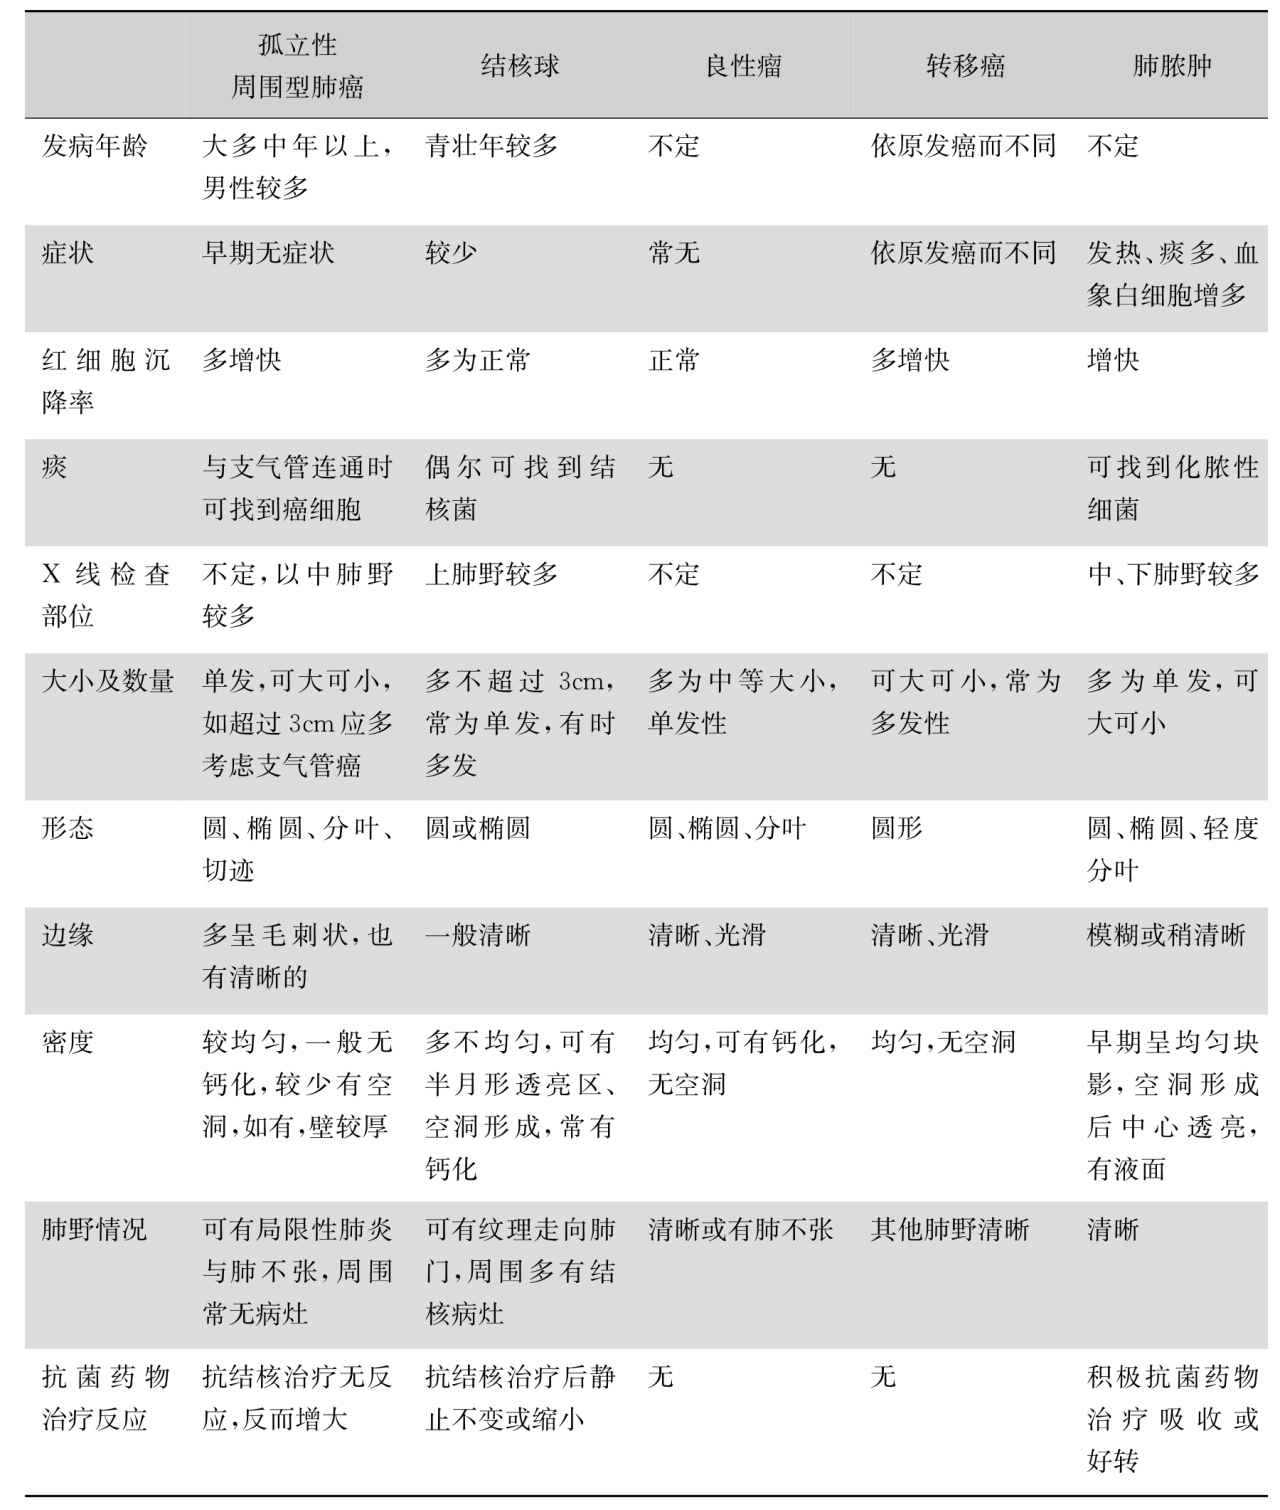
\includegraphics[width=5.98958in,height=7.0625in]{./images/Image00067.jpg}
\end{table}

\subsection{四、肺部化学感受器瘤}

化学感受器瘤是一种低度恶性肿瘤,临床上少见。原发部位为腹膜后、颈、肺等。X线表现为类圆形、密度均匀、边缘清楚致密阴影,单发者常为原发性,多发性双侧性者为转移性,原发瘤多位于腹膜后或颈部等;偶尔并发胸腔积液。诊断须依靠手术后活检。术前常被误诊为结核瘤、包虫病、胸膜间皮瘤等。

\subsection{五、肺部单发转移性肿瘤}

肺部单发转移性肿瘤少见,原发部位以消化道肿瘤最常见,亦可见于乳腺癌、宫颈癌、绒癌、肾癌、膀胱癌、骨肉瘤、鼻腺癌等。转移瘤较多发生于右肺,特别是右上肺。症状多为咳嗽、咯血、胸痛等。少数可无症状。有时转移到支气管的肿瘤,其临床表现如同原发性肺癌。痰脱落细胞检出率远较原发性肺癌为低。单发肺转移瘤与原发性肺癌的主要临床鉴别点为发现肺外原发肿瘤的存在。

近年有作者提到此瘤X线胸片特征为:①肺内较大的密度较高的团块阴影;②结构均匀,肿块内无钙化和空洞;③边缘明显,可有切迹,但无毛刺样改变;④肿块邻近无肺不张,周围无卫星灶与明显炎症浸润;⑤气管无移位。

CT能发现肺内0.4cm以下的微小细节,有助于诊断;鉴别困难者动态观察最好不超过2个月,必要时行CT导引下活组织穿刺检查确诊。PET/CT可发现肺外肿瘤灶。

\subsection{六、肺良性转移性平滑肌瘤病(PBML)}

良性转移性平滑肌瘤病(BML)为Streiner在1937年首次报道,多为PBML,大多数病理学家认同BML可能是良性子宫肌瘤发生远处血行转移所致。其病理特点为核分裂不活跃、细胞分化良好,无坏死的平滑肌瘤,瘤细胞多呈束状平行、编织状或漩涡状排列,无周围浸润性生长倾向,瘤组织内可见上皮细胞衬里的裂隙和腺样结构,可见增生的肺泡上皮向瘤内延伸及周围受挤压的肺泡结构,免疫组织化学染色结蛋白、波形蛋白、平滑肌蛋白阳性,雌激素受体(ER)及孕激素受体(PR)阳性。PBML胸部X线及CT多表现为双肺内多发结节,大小不等边界清楚,也有表现为粟粒性、空洞或囊肿样改变,极易误诊。大多发病女性有子宫肌瘤术后3个月至20年病史。大多无临床表现,偶有干咳、胸痛或呼吸困难等,通常因其他原因偶然发现。诊断需肺内结节活检病理学检查,根据镜下表现及免疫组织化学染色结果,结合病史而作出,良性子宫肌瘤与远处转移病灶为同一种组织是诊断本病的关键。抗性腺激素的内分泌治疗有效如三苯氧胺、芳香化酶抑制剂及黄体生成素释放激素。本病进展缓慢,预后较好。

\subsection{七、胸膜间皮瘤}

胸膜间皮瘤是一种少见的、由浆膜间皮细胞形成的肿瘤,可分为局限型与弥漫型二型。局限型可为良性或恶性。弥漫型均为恶性。局限性胸膜间皮瘤患者主诉多为胸痛、咳嗽、气喘、发热可伴有游走性关节痛及杵状指等。X线胸片显示胸部大小不等的球形或椭圆形阴影,密度深而均匀,边缘清楚光滑或轻度分叶,内无空洞或钙化,外无毛刺或脐凹,邻近肺野清晰。CT表现为密度均匀、边界光整、紧邻胸膜的孤立型类圆形块影。良性者常不大,有蒂。恶性者附近肋骨可有明显腐蚀性破坏。肿块可特别巨大,可占肺野的一半或大半,一般的肺癌或肺肉瘤极少有如此之大。国内有学者认为胸片或CT片上见患侧胸膜、纵隔胸膜紧邻的密度均匀、边界光整、孤立型类圆形块影应考虑到局限性胸膜间皮瘤之可能。胸膜活检、胸腔镜、经皮肺穿刺活检病理确诊,局限型胸膜间皮瘤治疗首选外科手术。

\subsection{八、支气管腺瘤}

支气管腺瘤是一种低度恶性肿瘤,约占支气管肿瘤的5\%左右。目前已废弃支气管腺瘤这一名称,采用支气管类癌、腺样囊性癌(圆柱瘤)和黏液表皮样癌的命名,并将此三类瘤归属肺癌分类中。发病年龄较早,在20~30岁之间,病变可长时间稳定而无明显发展,甚至生长停滞;患者一般健康状态良好。该瘤大多发生于大的支气管,周围型较少。腺瘤突出于管腔内可引起阻塞性肺不张,患者常因合并感染,以咯血、咳痰、胸痛等症状而就诊,经治疗后炎症消退;但因腺瘤在支气管内的可动性,使肺不张时重时轻。少数患者可有类癌综合征的表现。X线检查肿瘤在肺野呈圆形或分叶状、边缘清晰的阴影。最后确诊须依靠支气管镜直视下作病理活组织检查或开胸探查。

\subsection{九、肺部良性肿瘤}

\subsubsection{(一)肺错构瘤}

肺错构瘤为混合性良性肿瘤,以软骨为主要结构,此外尚有脂肪、结缔组织、腺体、骨质及淋巴组织。此瘤可发生于任何年龄,以40岁以上者居多。患者多无症状与体征,如肿瘤位于胸膜下可引起胸痛,位近肺门可压迫气管、支气管而引起咳嗽,呼吸困难,有时可引起咯血而易与肺结核球混淆。

在肺部孤立性球形病灶中,肺错构瘤有报告发生率仅次于肺癌、肺结核球、炎性假瘤而居第四位。X线表现为孤立性的、位于肺野外周的圆形或椭圆形阴影,边缘光滑锐利,体层片中可显示浅分叶状。约1/3病例有钙化点,“爆米花样钙化”为该病特征性表现。高精确度CT扫描发现病灶内钙化和脂肪密度区可提高诊断率,个别病灶位于支气管腔内。

肺错构瘤要与肺癌、结核球、硬化性血管瘤相鉴别:①肺错构瘤主要表现为边界清楚的软组织结节,无明显分叶及毛刺,CT平扫显示脂肪成分及典型的爆米花样钙化时可以明确诊断,增强扫描后病变呈轻度强化,强化程度小于20HU。②肺癌结节形状通常不规整,可见深浅不一的分叶和毛刺,可有空泡征、血管集束征及胸膜凹陷征等,结节内无脂肪,少见钙化。如出现钙化则多是肿瘤内部散在分布的沙粒或面沙样钙化,且钙化范围不是很大。增强后强化程度>20HU,可见肺门、纵隔淋巴结肿大及肺内、外转移。③结核球是由纤维包膜包裹干酪样物质所构成,其内也可见钙化,多呈斑片状或不规则形钙化,但结核球有一定的好发部位(双肺上叶尖后段和下叶背段),瘤体边界可不光滑。瘤内可有小空洞存在,瘤周常有卫星病灶。④硬化性血管瘤也是一种肺内少见的良性肿瘤,多表现为边界清楚,内部无脂肪成分,可见钙化,但增强以后呈明显强化,错构瘤则呈轻度强化。

肺错构瘤为局部支气管发育异常,大多无症状,几乎不发生恶变,但往往又难与肺癌相鉴别且也有并发肺癌的危险性;肿瘤逐渐增大压迫或阻塞支气管腔易致相应肺叶、肺段炎症或肺不张,因而主张手术治疗。

\subsubsection{(二)支气管软骨瘤}

支气管软骨瘤来源于气管、支气管和细支气管的软骨,是少见的肺部良性肿瘤。其胸部X线呈椭圆形或圆形高密度影,边缘清晰、光滑,可有分叶,有时可见钙化灶。软骨瘤生长缓慢,临床症状不明显,当肿瘤增大时可导致阻塞远端肺组织继发感染。支气管软骨瘤需与肺错构瘤、肺部恶性肿瘤鉴别。诊断主要根据手术后标本病理学检查。

\subsection{十、孤立性肺囊肿}

孤立性肺囊肿可表现为气囊肿、气液囊肿和液囊肿。液囊肿在X线照片上呈一圆形或卵圆形阴影,密度均匀,边缘清晰,周围的肺组织无浸润病变,囊肿长期无改变,此种情况一般与肿瘤不易混淆。临床常因继发感染出现症状,此时与肺脓肿、肺结核、肺包虫囊肿不易区别。后者有一定的地区性,血内嗜酸性粒细胞增多,包虫抗原皮内试验及补体结合试验大多阳性。B超、CT、MRI检查有助于囊内容物的定性,有较高的诊断价值。纤维支气管镜检查结合病理,可协助确诊。

\subsection{十一、肺动静脉瘘}

本病是先天性肺血管的血管瘤样畸形,也可为获得性,临床上十分罕见。病理上分囊状肺动静脉瘘和弥漫型肺小动静脉瘘。囊状肺动静脉瘘可表现为单发或多发肺部球形病灶。

患者可有发绀、杵状指(趾)及红细胞增多症,如动静脉瘘相当大和位置较浅,可在相应的胸壁部位听到来回性血管杂音,有时尚可能触及震颤。肺动静脉瘘发病常与遗传性出血性毛细血管扩张症有关。

X线检查在诊断上起重要的作用,其特点是:①呈圆形或卵圆形致密阴影,直径由0.5cm至数厘米不等,较多发生于肺的中部或下部;②在圆形阴影和肺门之间可见条索状阴影,此为输入和输出的血管,透视下可见圆形阴影有搏动现象;③作Valsalva动作(紧闭声门作持续而用力的呼气),由于胸膜腔内压升高,流入胸腔的血液减少,可见圆形阴影显著缩小。肺动脉造影是确诊肺动静脉瘘的可靠方法,可明确病变部位、形态、累及的范围及程度,囊状肺动静脉瘘可见瘤囊随肺动脉的充盈显影,引流肺静脉显影早于正常肺静脉,供血动脉及引流静脉可为单支或多支;瘤囊内可见分隔,对比剂排空延迟。弥漫型肺动静脉瘘表现为多发“葡萄串”样小血池充盈,病变部位肺静脉提前显影。超声心动图声学造影、肺灌注核素扫描可协助诊断。螺旋CT及其三维重建和MRI及增强3D-SGPR扫描均可清晰地显示出肺动静脉瘘的全貌,并且具无创性,有人认为它们优于肺动脉造影。

肺动静脉瘘可误诊为肺结核球或支气管癌,但无钙化或空洞形成,或可发现与肺门连接的血管,长期经过全身情况佳良,结合上述的其他特点,一般不难鉴别。

\subsection{十二、肺隔离症}

肺隔离症是一种少见的先天性肺发育异常,其解剖学特点为由主动脉的异常分支所供应的、无功能的、和支气管不相通或仅有一小口与之相通的囊性肺组织,故称肺隔离症。肺隔离症的系列表现为:①隔离或发育不良的肺肿块;②异常供血动脉;③异常引流静脉;④与气管或胃肠道沟通;⑤大量肺组织发育异常;⑥横膈缺损。根据其与脏层胸膜的关系,可分为叶内型与叶外型,前述表现的后三项以叶外型多见。临床上则以叶内型较常见,病变在肺叶内。常位于下叶后基底段,左下肺多见。本病多见于青少年,如无继发感染,则无症状,于体检X线检查偶然发现。叶内型因与支气管相通,易合并肺部感染,常表现为反复咳嗽、咳浓痰、发热、胸闷、胸痛等,少数患者可反复咯血;叶外型多无临床症状。

胸片是诊断肺隔离症最基本、首选的方法。X线表现为肺下叶后基底段实性或囊性肿块,边缘多较清楚。当合并周围肺组织感染时,边缘模糊不清,部分囊内可见液平面。经抗炎治疗后病变可缩小、边缘变清楚,但病变长期不消失。少数患者只表现为单侧下肺肺血增多、粗或基本正常。B超、CT、MRI对显示异常动脉有重要诊断价值,而主动脉造影对本病确诊有决定意义。本病有时与支气管扩张、先天性肺囊肿合并感染、肺癌、肺脓肿、肺炎性假瘤等难以鉴别,且有潜在大咯血可能,应及时手术探查或行CT血管造影(CTA)、三维磁共振血管成像明确诊断。

目前,肺隔离症的影像学确诊主要在于显示其异常的供血动脉和引流静脉;此外,此病主要通过手术治疗,故对于显示其异常的供血动脉和引流静脉尤为重要,这样可避免术中大出血。肺隔离症的血液供应通常来自胸内降主动脉发出的异常分支,10\%~15\%来自腹主动脉和腹腔动脉发出的异常分支,也可来自主动脉弓、无名动脉、内乳动脉、肋间动脉、锁骨下动脉、膈动脉或肾动脉等发出的分支。肺隔离症的供血血管通常为1支,此时血管较粗,直径约在0.5~2.0cm之间;也可为多条,最多达6条,此时血管较细,直径在0.3cm以下。肺叶内型肺隔离症的静脉通常回流到下肺静脉,有时回流到奇静脉、半奇静脉,偶有回流到肋间静脉或无名静脉。肺叶外型肺隔离症的静脉多回流到奇静脉和半奇静脉,或经腔静脉至右房,25\%可回流到肺静脉。

重建的三维(3D)磁共振血管成像(MRA)图像能更好地显示异常供血动脉的起源、行程、分支及其静脉回流。辅以平扫MRI显示隔离肺组织团块的结构、位置以及与支气管或胃肠道沟通的关系,有助于疾病确诊和手术方案制订。有学者认为其优于动脉造影。

\subsection{十三、胆固醇肺炎}

本病罕见,病程慢性,患者有发热、咳嗽、多痰、胸痛、偶有咳血等症状,胸部X线可表现为肺内肿块、肺实变或不张等多种表现。CT可见肿块或肺实变区内类似脂肪的低衰减区,是胆固醇肺炎的特点。如为球形病灶,须经手术探查活检方能与结核球、肺癌等鉴别。胆固醇肺炎的病理特征为肺泡内含大量胆固醇巨噬细胞。

\protect\hypertarget{text00091.html}{}{}

\section{参考文献}

1.潘道刚,等.54例肺部孤立性圆形病灶临床分析.临床肺科杂志,2010,15(8):1186

2.中华医学会中华中医药学会.重症急性呼吸综合征(SARS)诊疗方案.卫生部网2003;9.30.

3.柏松.球形肺炎的影像学诊断与鉴别诊断.实用临床医学,2009,10(7):101-102,104

4.刘丽芬,等.重症急性呼吸综合征CT表现及其CT动态观察的意义.中国医学影像技术,2003,19(7):807-809

5.向阳,等.肺曲霉菌病的外科治疗.中华结核和呼吸杂志,2004,27(1):68-69

6.潘会明,等.三峡库区肺吸虫病病例报道及流行病学调查.中国寄生虫病防治杂志,2001,14(4):4-5

7.陈奕鹏,等.肺错构瘤的综合影像学诊断.影像诊断与介入放射学,2009,18(6):292-294

8.夏前明,等.先天性支气管肺囊肿15例分析.中国呼吸与危重症监护杂志,2002,1(3):182-184

9.程晓光,等.SARS的胸部CT早期表现.中华放射学杂志,2003,37(9):790-794

10.陈晓,等.肺良性转移性平滑肌瘤病一例.中华结核和呼吸杂志,2013;36(2):128-129

11.黄志勇,等.肺硬化性血管瘤五例报告.临床外科杂志,1999,7(2):107

12.肖运平,等.叶内型肺隔离症的影像学表现与手术病理对照.实用放射学杂志,2010,26(11):1600-1603.

13.宾怀有,等.7例胆固醇肺炎的影像学诊断.广西医学,2007,29(5):755-756.

\protect\hypertarget{text00092.html}{}{}

